\subsection{Grundlegende Anpassungen des Datenbankschemas}
Die Umsetzung der Funktionalen Anforderungen eins bis neun (vgl. Tabelle \eqref{tab:funktionale_anforderungen}) haben eine große Bedeutung zur Lösung 
der Forschungsfrage. 
Sie basieren auf den theoretischen Erkenntnissen bezüglich Energiebilanzierung und sollen sicher stellen dass das Bilanzraumkonzept auf dem aktuellen Stand der Wissenschaft 
in diesem Forschungsgebiet gerecht wird.
Somit bilden diese Anforderungen die Grundlage des entworfenen Konzepts.

\begin{figure}[H]
    \centering
    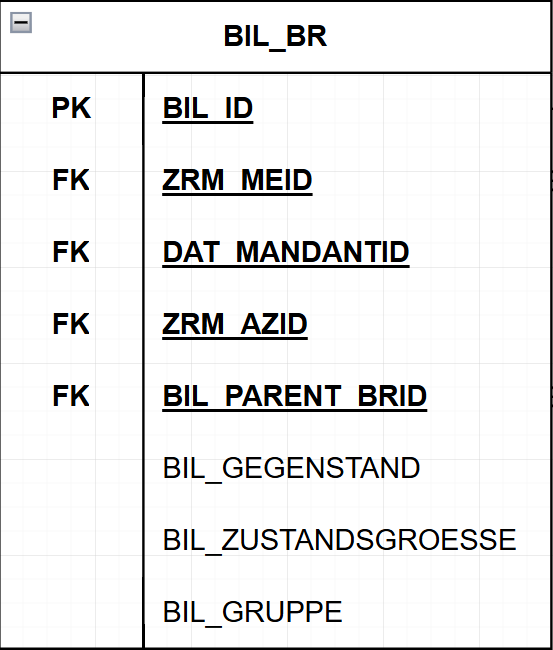
\includegraphics[width=0.4\textwidth]{../../Ressourcen/Abbildungen/Konzept/BIL_BR.png}
    \caption{Tabelle BIL\_BR. (Eigene Darstellung)}
    \label{fig:BIL_BR}
\end{figure}

Die Datenbanktabelle BIL\_BR (vgl. Abbildung \eqref{fig:BIL_BR}) steht im Zentrum der grundlegenden Datenbankstruktur und stellt den Bilanzraum dar.
In der Datenbanktabelle wird mit der Spalte BIL\_GEGENSTAND der Untersuchungsgegenstand des Bilanzraums definiert und somit die Funktionale Anforderung 
zwei (vgl. Tabelle \eqref{tab:funktionale_anforderungen}) erfüllt.
Über die Relation zur Tabelle ZRM\_ME über die Spalte ZRM\_MEID wird die Einheit der Zustandsgröße des Bilanzraums definiert.
% TODO: Constraint kWh
Diese Relation dient der Erfüllung der funktionalen Anforderung fünf da mit der Definition dieser Einheit die Einheiten der zu- und abfließenden Energieströme und 
der Energiequellen und -senken möglich ist.
Die Relation zur Tabelle ZRM\_AZ durch die Spalte ZRM\_AZID dient der Erfüllung der funktionalen Anforderung drei (vgl. Tabelle \eqref{tab:funktionale_anforderungen}) und nutzt die 
in EDM-EMS-Prophet® bestehende Tabelle zur Festlegung des Zeitintervalls des Bilanzraums.
Die in Anforderung neun (vgl. Tabelle \eqref{tab:funktionale_anforderungen}) festegelegte Definierbarkeit der Bilanzraumgrenzen nach den von der E DIN ISO 50006:2024-07 
festgelegten Kriterien (vgl. Abbildung \eqref{fig:EnPI_Grenzniveaus}) wird durch die Spalten DAT\_MANDANTID, BIL\_GRUPPE und BIL\_GEGENSTAND erfüllt.
Die Abgrenzung auf Organisatorischem Niveau kann durch die festlegung eines Mandanten durch die in DAT\_MANDANTID realisierte relation zur Tabelle 
DAT\_MANDANT definiert werden. 
Die Systembezogene Abgrenzung kann durch die definition einer Gruppen in der Spalte BIL\_GRUPPE durchgeführt werden. 
Die Abgrenzung auf einzelnem Niveau kann durch die definition des Untersuchungsgegenstands durch BIL\_GEGENSTAND durchgeführten werden.
Um die in Anforderung sieben beschriebene Disaggregation von Bilanzräumen zu realisieren stellt die Spalte BIL\_PARENT\_BRID eine reflexive Relation zur Tabelle BIL\_BR 
dar und ermöglicht somit eine rekursive Disaggregation eines Bilanzraums in mehrere Teilbilanzräume welche in der genannten Spalte auf den Vaterbilanzraum verweisen. 
% TODO: Constraint zur verhinderung von Kreisen

\begin{figure}[H]
    \centering
    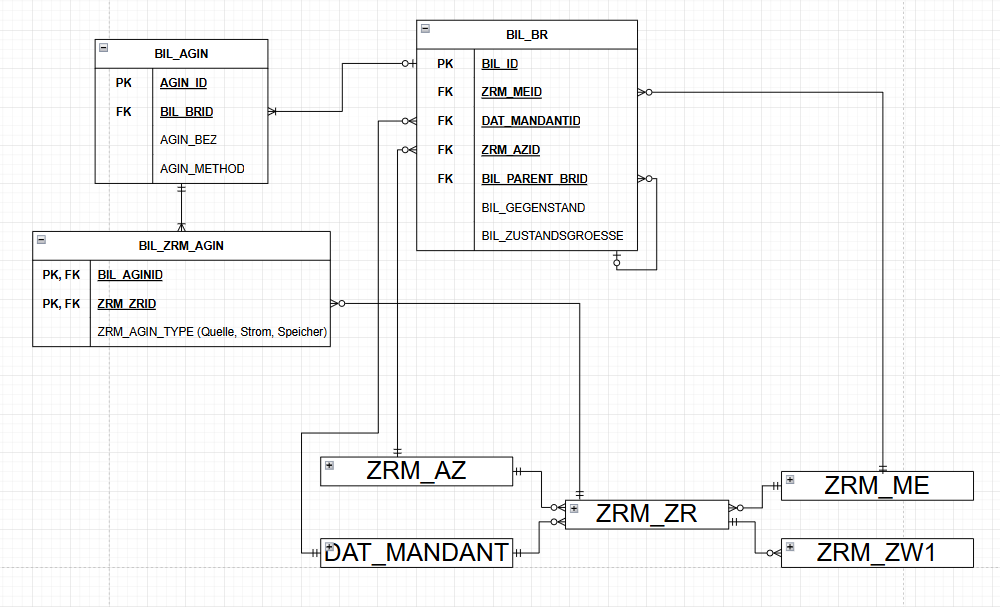
\includegraphics[width=0.7\textwidth]{../../Ressourcen/Abbildungen/Konzept/BIL_AGIN.png}
    \caption{Tabelle BIL\_AGIN. (Eigene Darstellung)}
    \label{fig:BIL_AGIN}
\end{figure}
